% =============================================================================
% 4 METODOLOGIA — primeira versão (16/11/2026).
% Fontes: docs/decisions.md (D-001 a D-008); src/tccsql/; scripts/;
% data/datasets/commercial/; artifacts/data_assessment/report.md;
% artifacts/raw/ (runs 22e3f8ce e 07a25f55).
% Fluxo descrito segundo runner.py (semantic = catalog + YAML), não segundo
% docs/architecture.md, que documenta o desenho antigo de duas condições.
% =============================================================================
\chapter{Metodologia}
\label{cap:metodologia}

Esta seção descreve o experimento conduzido para medir o efeito da
representação do esquema sobre a correção das consultas SQL geradas por um
agente baseado em modelo de linguagem. São apresentados o delineamento
experimental, a base de dados, as três condições de contexto comparadas, o
agente, os modelos, o banco de perguntas, os controles, o critério de
correção e a análise estatística. Ao final, registra-se a trajetória de
decisões metodológicas que levou ao protocolo definitivo e o ambiente
necessário para reproduzi-lo.

% -----------------------------------------------------------------------------
\section{Delineamento do experimento}
\label{sec:delineamento}

O estudo é um experimento controlado com medidas repetidas: cada pergunta do
banco é apresentada ao agente em todas as condições de contexto, de modo que
cada pergunta funciona como seu próprio controle. Essa escolha elimina a
variação entre perguntas da comparação entre condições e permite o uso de
testes pareados.

A variável independente é a representação do esquema fornecida ao modelo,
em três níveis progressivamente aditivos:
\begin{alineas}
  \item \textbf{técnica}: a definição textual das tabelas, colunas, chaves
        primárias e chaves estrangeiras;
  \item \textbf{catálogo}: a representação técnica acrescida de descrições
        por tabela e por coluna;
  \item \textbf{semântica}: o catálogo acrescido de uma camada semântica com
        regras de grão, regras temporais, regras referenciais, sinônimos e
        orientações de estilo de resposta.
\end{alineas}

Cada nível contém integralmente o anterior. Assim, a diferença entre
técnica e catálogo isola o efeito das descrições de coluna, e a diferença
entre catálogo e semântica isola o efeito das regras da camada semântica
(\autoref{fig:delineamento}).

\begin{figure}[htb]
  \centering
  \caption{Condições de contexto progressivamente aditivas}
  \label{fig:delineamento}
  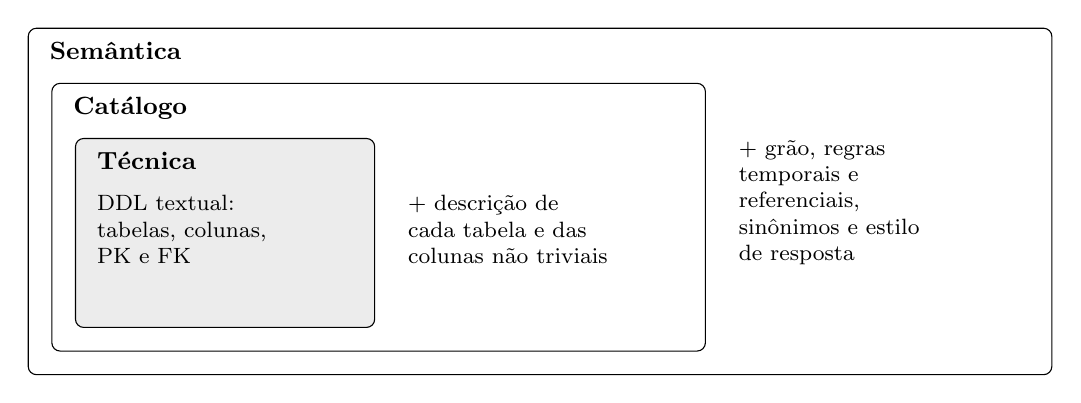
\begin{tikzpicture}[font=\small]
    % caixas aninhadas com coordenadas fixas (cm)
    \draw[rounded corners=3pt] (0,0) rectangle (13,4.4);
    \draw[rounded corners=3pt] (0.3,0.3) rectangle (8.6,3.7);
    \draw[rounded corners=3pt, fill=gray!15] (0.6,0.6) rectangle (4.4,3.0);
    \node[anchor=north west, font=\small\bfseries] at (0.15,4.35) {Semântica};
    \node[anchor=north west, font=\small\bfseries] at (0.45,3.65) {Catálogo};
    \node[anchor=north west, font=\small\bfseries] at (0.75,2.95) {Técnica};
    \node[anchor=north west, align=left, font=\footnotesize] at (0.75,2.4)
      {DDL textual:\\tabelas, colunas,\\PK e FK};
    \node[anchor=north west, align=left, font=\footnotesize] at (4.7,2.4)
      {+ descrição de\\cada tabela e das\\colunas não triviais};
    \node[anchor=north west, align=left, font=\footnotesize] at (8.9,3.1)
      {+ grão, regras\\temporais e\\referenciais,\\sinônimos e estilo\\de resposta};
  \end{tikzpicture}
  \fonte{Elaborado pelo autor.}
\end{figure}

As variáveis dependentes são:
\begin{alineas}
  \item \textbf{correção}, variável binária que indica se a consulta gerada
        executa e devolve o mesmo resultado da consulta de referência
        (\autoref{sec:avaliacao});
  \item \textbf{latência do modelo}, o tempo de parede da chamada ao
        provedor, em milissegundos (\autoref{sec:analise}).
\end{alineas}

Permanecem constantes entre as condições: o agente, o modelo, as perguntas,
o \textit{snapshot} da base de dados, os parâmetros de geração e o critério
de correção. A hipótese nula é a de que não há diferença de acurácia entre
as condições; a alternativa é bilateral, de forma que o estudo pode detectar
tanto melhora quanto piora.

% -----------------------------------------------------------------------------
\section{Fonte de dados}
\label{sec:fonte-dados}

\subsection{Seleção e autorização}
\label{sec:selecao-base}

Três conjuntos de dados candidatos foram avaliados localmente, apenas por
estrutura e estatísticas agregadas (contagens, cabeçalhos, tipos, nulos e
duplicidades), sem exposição de valores de linha. O resultado da avaliação
está resumido no \autoref{qua:bases}.

\begin{quadro}[htb]
  \centering
  \caption{Classificação das bases candidatas}
  \label{qua:bases}
  \begin{tabularx}{\textwidth}{|l|l|X|}
    \hline
    \textbf{Base} & \textbf{Classificação} & \textbf{Justificativa} \\ \hline
    Comercial & Usar com transformações & Autorização confirmada; 11 tabelas
      relacionadas; exige normalização de XLSX para PostgreSQL. \\ \hline
    Financeiro & Não usar & Autorização específica e privacidade não
      confirmadas. \\ \hline
    CSVs sintéticos fragmentados & Não usar & Não formam um
      \textit{snapshot} relacional íntegro. \\ \hline
  \end{tabularx}
  \fonte{Elaborado pelo autor a partir de \arq{artifacts/data_assessment/report.md}.}
\end{quadro}

A base escolhida, denominada \arq{commercial}, é um recorte comercial
descaracterizado. Em 26 de setembro de 2026, o responsável pelos dados
confirmou a descaracterização e autorizou o uso acadêmico local
(decisão D-001). A base financeira foi excluída por falta de confirmação
específica. Um conjunto sintético (\arq{synthetic_commercial}) foi mantido
apenas para os testes automatizados do código e não participa do
experimento.

A opção por uma base real descaracterizada, em vez de um \textit{benchmark}
acadêmico com esquema preparado para avaliação, é deliberada. A base carrega
características típicas de dados comerciais autênticos: referências órfãs
entre tabelas, datas registradas por extenso em português, nomes de coluna
que misturam termos de negócio e convenções técnicas, e medidas
monetárias em grãos diferentes. Essas características tornam o teto de
acurácia mais baixo, mas aproximam a medição do cenário em que agentes de
consulta são efetivamente empregados.

\subsection{Transformação para o modelo relacional}
\label{sec:transformacao}

As 11 planilhas XLSX de origem foram lidas sem modificação e normalizadas em
um esquema PostgreSQL com 11 tabelas, descritas no \autoref{qua:tabelas}.
As datas de emissão, registradas em português por extenso (por exemplo,
``terça-feira, 13 de dezembro de 2016''), foram convertidas para o tipo
\arq{date} durante a carga. Após a carga, a base contém 10.931 pedidos e
246.737 itens de pedido, com datas de emissão entre 18 de janeiro de 2016 e
26 de fevereiro de 2026.

\begin{quadro}[htb]
  \centering
  \caption{Tabelas do esquema \arq{commercial}}
  \label{qua:tabelas}
  \begin{tabularx}{\textwidth}{|l|l|X|}
    \hline
    \textbf{Tabela} & \textbf{Papel} & \textbf{Conteúdo e grão} \\ \hline
    \arq{orders} & Fato & Cabeçalho de pedido, uma linha por pedido \\ \hline
    \arq{order_items} & Fato & Item de pedido, N linhas por pedido \\ \hline
    \arq{targets} & Fato & Metas e realizado por representante e período \\ \hline
    \arq{customers} & Dimensão & Clientes \\ \hline
    \arq{representatives} & Dimensão & Representantes de vendas \\ \hline
    \arq{products} & Dimensão & Produtos cadastrados \\ \hline
    \arq{collections} & Dimensão & Coleções de produto, com vigência \\ \hline
    \arq{families} & Dimensão & Famílias de produto, agrupadas por coleção \\ \hline
    \arq{groups} & Dimensão & Grupos de classificação de produto \\ \hline
    \arq{subgroups} & Dimensão & Subgrupos, aninhados em grupos \\ \hline
    \arq{lines} & Dimensão & Linhas de produto \\ \hline
  \end{tabularx}
  \fonte{Elaborado pelo autor a partir de \arq{data/datasets/commercial/schema.sql}
    e \arq{catalog_context.sql}.}
\end{quadro}

\pendente{figura com diagrama entidade-relacionamento simplificado (opcional)}

O principal risco analítico do esquema é a relação de um para muitos entre
\arq{orders} e \arq{order_items}: somar uma medida do cabeçalho do pedido
após juntar os itens multiplica o valor pelo número de itens. Outro risco
é a coexistência de várias datas com semânticas distintas (emissão, entrega
prevista, cadastro de cliente, vigência de coleção e período de meta).

A primeira carga falhou porque a tabela \arq{subgroups} continha
referências a grupos inexistentes. Dados comerciais reais contêm
referências órfãs, e esse comportamento foi considerado parte do objeto de
estudo. Para preservar a fonte exatamente como autorizada, as declarações
\arq{REFERENCES} foram removidas do esquema (decisão D-004): as tabelas
mantêm nomes, tipos, chaves primárias e restrições \arq{NOT NULL}, mas o
PostgreSQL não valida a integridade referencial. A descrição textual das
relações (``FK $\rightarrow$ tabela'') continua sendo apresentada ao modelo.
A extensão do fenômeno é visível na tabela de pedidos: dos 10.931 pedidos
com cliente informado, 10.375 têm correspondência na tabela de clientes.

\subsection{Privacidade}
\label{sec:privacidade}

Nenhum valor de linha da base é enviado ao provedor do modelo
(decisão D-003). O modelo recebe apenas a descrição do esquema, o contexto
da condição e a pergunta. O agente não recebe amostras do resultado das
consultas que gera. Quando uma consulta
falha, o agente recebe somente a mensagem de erro de validação ou de
execução. A comparação entre o resultado gerado e o de referência é feita
localmente.

% -----------------------------------------------------------------------------
\section{Condições de contexto}
\label{sec:condicoes}

As três condições correspondem a três arquivos de texto mantidos sob
controle de versão e congelados por \textit{hash} (\autoref{sec:controles}).
O \autoref{qua:condicoes} resume o conteúdo de cada uma, e a
\autoref{tab:tamanho-contexto} mostra o tamanho do prompt resultante.

\begin{quadro}[htb]
  \centering
  \caption{Conteúdo de cada condição de contexto}
  \label{qua:condicoes}
  \begin{tabularx}{\textwidth}{|l|l|X|}
    \hline
    \textbf{Condição} & \textbf{Arquivo(s)} & \textbf{Conteúdo} \\ \hline
    Técnica & \arq{technical_context.sql} & Uma linha por tabela com colunas,
      chave primária e chaves estrangeiras (``FK $\rightarrow$ tabela''),
      sem descrições. \\ \hline
    Catálogo & \arq{catalog_context.sql} & O mesmo esquema, uma coluna por
      linha, com descrição de cada tabela e das colunas não triviais
      (valores monetários, contagens e datas), no formato de comentários
      de catálogo. \\ \hline
    Semântica & \arq{catalog_context.sql} + \arq{semantic_context.yaml} &
      O catálogo seguido do bloco ``SEMÂNTICA'', com: campos monetários e de
      contagem por tabela; regras de grão; regras temporais; regras
      referenciais; sinônimos em português; estilo de resposta. \\ \hline
  \end{tabularx}
  \fonte{Elaborado pelo autor a partir de \arq{data/datasets/commercial/}
    e \arq{src/tccsql/experiment/runner.py}.}
\end{quadro}

A condição técnica é análoga a fornecer ao modelo apenas a definição das
tabelas. A condição de catálogo é análoga aos comentários
\arq{COMMENT ON TABLE} e \arq{COMMENT ON COLUMN} mantidos em catálogos de
dados corporativos. A condição semântica é análoga a uma camada semântica,
que adiciona definições de métricas, grão, dimensões temporais e regras de
relacionamento. A correspondência entre cada seção do contexto semântico e
as ferramentas industriais é discutida na \autoref{sec:industriais}.

O contexto semântico é organizado em sete blocos:
\begin{alineas}
  \item \arq{money_fields} e \arq{count_fields}: definição de cada campo
        monetário e de contagem, por tabela;
  \item \arq{grain_rules}: o grão de cada tabela de fato e a proibição de
        somar \arq{orders.total_amount} após juntar os itens;
  \item \arq{temporal_rules}: qual coluna de data usar para emissão,
        entrega prevista, meta, vigência de coleção e cadastro de cliente;
  \item \arq{referential_rules}: o aviso de que há referências órfãs e a
        regra de usar \arq{IS NOT NULL} para ``Y informado'' e \arq{JOIN}
        para ``associado a Y existente'';
  \item \arq{synonyms}: termos de negócio em português (vendedor,
        representante, pedido, item, produto, faturamento) mapeados para
        tabelas e colunas;
  \item \arq{response_style}: devolver apenas as colunas pedidas,
        devolver um escalar quando não há agrupamento e não aplicar
        conversões de tipo desnecessárias;
  \item um cabeçalho com o domínio da base e a restrição de privacidade.
\end{alineas}
O conteúdo integral dos três contextos está no Apêndice~\ref{ap:contextos}.

\begin{table}[htb]
  \centering
  \caption{Tamanho do contexto por condição}
  \label{tab:tamanho-contexto}
  \begin{tabular}{lrrr}
    \toprule
    \multirow{2}{*}{Condição} & \multirow{2}{*}{Arquivo (bytes)} &
      \multicolumn{2}{c}{Tokens de entrada (mediana)} \\
    \cmidrule(lr){3-4}
     & & gpt-oss-120b & qwen3.8-27b \\
    \midrule
    Técnica   & 1.392 & 434 & 387 \\
    Catálogo  & 3.001 & 885 & 858 \\
    Semântica & 3.001 + 2.992 & 1.722 & 1.716 \\
    \bottomrule
  \end{tabular}
  \fonte{Elaborado pelo autor. Bytes dos arquivos em
    \arq{data/datasets/commercial/}; tokens de entrada informados pelo
    provedor em cada chamada, mediana sobre todas as tentativas das rodadas
    \arq{22e3f8ce} e \arq{07a25f55} (\arq{artifacts/raw/}).}
\end{table}

A descrição das colunas no catálogo e as definições dos campos no contexto
semântico se sobrepõem parcialmente. Essa sobreposição é intencional: o
nível semântico precisa conter todo o catálogo para que o desenho seja
aditivo, e a camada semântica de ferramentas industriais também repete
definições de campo ao lado das regras.

Um quarto arquivo do conjunto de dados, \arq{business_rules.yaml}, registra
as regras de negócio usadas na elaboração das perguntas e não é enviado ao
modelo em nenhuma condição.

% -----------------------------------------------------------------------------
\section{Agente de tradução para SQL}
\label{sec:agente}

O agente foi mantido deliberadamente simples para que o contexto fosse a
única fonte de variação. Ele faz uma única chamada ao modelo por tentativa,
sem exemplos (\textit{few-shot}), sem ferramentas, sem recuperação de
documentos e sem encadeamento de chamadas. O \textit{prompt} é composto por
uma mensagem de sistema fixa e uma mensagem de usuário com o contexto da
condição e a pergunta (\autoref{lst:prompt}).

\begin{lstlisting}[caption={Estrutura do \textit{prompt} enviado ao modelo},label={lst:prompt}]
[system]
Você é um agente text-to-SQL PostgreSQL. Responda somente com uma única
consulta SELECT ou WITH terminada em SELECT. Não explique.

[user]
ESQUEMA:
<contexto da condição: técnica, catálogo ou semântica>

PERGUNTA:
<pergunta em português>
SQL:
\end{lstlisting}
\fonte{\arq{src/tccsql/agent/text2sql.py}.}

O fluxo de execução de uma pergunta em uma condição é mostrado na
\autoref{fig:fluxo}. A resposta do modelo é reduzida ao bloco de código
SQL, quando presente, e passa por um validador sintático baseado na
biblioteca \textit{sqlglot}. O validador aceita uma única instrução, que
deve ser \arq{SELECT} ou \arq{WITH} terminado em \arq{SELECT}, rejeita
comandos de escrita e de definição de dados e restringe o acesso ao
esquema \arq{public}. A consulta validada é executada em uma transação
somente leitura, com um usuário de banco que possui apenas permissão de
leitura e tempo limite de 5 segundos por instrução.

\begin{figure}[htb]
  \centering
  \caption{Fluxo de execução de uma pergunta em uma condição}
  \label{fig:fluxo}
  \begin{tikzpicture}[
      font=\footnotesize, node distance=0.45cm and 0.5cm,
      caixa/.style={draw, rounded corners=2pt, align=center, minimum height=0.9cm, text width=2.0cm},
      seta/.style={-{Stealth[length=2mm]}}]
    \node[caixa] (q) {Pergunta +\\contexto};
    \node[caixa, right=of q] (m) {Modelo\\(Groq)};
    \node[caixa, right=of m] (v) {Validação\\somente\\leitura};
    \node[caixa, right=of v] (e) {Execução\\PostgreSQL};
    \node[caixa, below=1.1cm of e] (c) {Comparação\\com o gold};
    \node[caixa, left=of c] (g) {Execução do\\SQL de\\referência};
    \node[caixa, right=0.5cm of c, text width=1.6cm] (r) {Registro\\bruto};
    \draw[seta] (q) -- (m);
    \draw[seta] (m) -- (v);
    \draw[seta] (v) -- (e);
    \draw[seta] (e) -- (c);
    \draw[seta] (g) -- (c);
    \draw[seta] (c) -- (r);
    \draw[seta, dashed] (v.north) -- ++(0,0.5) -| node[pos=0.25, above] {erro: nova tentativa (até 3)} (m.north);
    \draw[seta, dashed] (e.north) -- ++(0,0.8) -| (m.110);
  \end{tikzpicture}
  \fonte{Elaborado pelo autor a partir de \arq{src/tccsql/experiment/runner.py}.}
\end{figure}

Se a validação ou a execução falhar, o agente faz uma nova tentativa, até o
limite de três tentativas por pergunta e condição. A nova chamada repete a
mensagem de sistema e a mensagem com contexto e pergunta, acrescida de uma
mensagem com o erro técnico (``A tentativa anterior falhou tecnicamente:
\textit{erro}. Corrija e responda somente SQL.''). A consulta que falhou
não é reenviada ao modelo. Uma consulta que executa sem erro encerra as
tentativas, mesmo que o resultado esteja incorreto: o agente não recebe
nenhum sinal sobre a correção do resultado, apenas sobre falhas técnicas.

% -----------------------------------------------------------------------------
\section{Modelos e parâmetros}
\label{sec:modelos}

Foram usados dois modelos de pesos abertos de famílias distintas, ambos
servidos pela camada gratuita da API da Groq, compatível com a interface da
OpenAI (\autoref{tab:modelos}). O modelo principal é o
\arq{openai/gpt-oss-120b}. O \arq{qwen/qwen3.8-27b}, menor e de outra
família, foi adicionado para avaliar se o efeito depende do modelo
(decisão D-007). O identificador do modelo devolvido pelo provedor é gravado
em cada registro bruto.

\begin{table}[htb]
  \centering
  \caption{Modelos avaliados e parâmetros de geração}
  \label{tab:modelos}
  \begin{tabular}{lll}
    \toprule
    Item & Modelo principal & Réplica \\
    \midrule
    Identificador & \arq{openai/gpt-oss-120b} & \arq{qwen/qwen3.8-27b} \\
    Família & GPT-OSS (OpenAI) & Qwen (Alibaba) \\
    Parâmetros & 120 bilhões & 27 bilhões \\
    Provedor & Groq (camada gratuita) & Groq (camada gratuita) \\
    \arq{temperature} & 0 & 0 \\
    \arq{max_tokens} & 800 & 800 \\
    Rodada da coleta final & \arq{22e3f8ce} (16/11/2026) & \arq{07a25f55} (14/11/2026) \\
    \bottomrule
  \end{tabular}
  \fonte{Elaborado pelo autor a partir de \arq{src/tccsql/experiment/runner.py},
    \arq{docs/decisions.md} e \arq{artifacts/raw/}.}
\end{table}

\pendente{citar a fonte primária (model card) da contagem de parâmetros de cada modelo}

A temperatura zero reduz a variabilidade da geração, mas não a elimina:
o código não fixa semente (\textit{seed}) na requisição, e provedores de
inferência não garantem saída idêntica entre chamadas. Essa limitação é
discutida na \autoref{sec:validade}.

O uso de modelos abertos servidos gratuitamente é uma escolha de projeto:
o experimento inteiro roda sem custo financeiro e sem dependência de
plataformas proprietárias de dados ou de modelos, o que permite que
qualquer pesquisador o reproduza ou o estenda com outros modelos.

% -----------------------------------------------------------------------------
\section{Banco de perguntas}
\label{sec:perguntas}

O banco tem 50 perguntas em português: 40 para a coleta final e 10 para o
estudo piloto. Os enunciados dos dois conjuntos são distintos, embora três
perguntas do piloto tenham a mesma consulta de referência de perguntas
finais, com outra redação. As perguntas da coleta final se distribuem
igualmente em quatro categorias (\autoref{tab:perguntas}). Cada pergunta
tem identificador, categoria, enunciado, consulta SQL de referência
(\textit{gold}), tolerância numérica e um indicador de se a ordem das linhas
importa para a correção. Nas 40 perguntas finais, a tolerância é
$10^{-6}$ e a ordem das linhas não é considerada.

\begin{table}[htb]
  \centering
  \caption{Distribuição das perguntas por categoria}
  \label{tab:perguntas}
  \begin{tabularx}{\textwidth}{lccX}
    \toprule
    Categoria & Final & Piloto & Exemplo (coleta final) \\
    \midrule
    Filtros e agregações & 10 & 3 & ``Quantos clientes há na base?'' \\
    Relacionamentos & 10 & 3 & ``Quantos pedidos têm cliente associado?'' \\
    Temporal & 10 & 2 & ``Quantos pedidos foram emitidos em cada ano?'' \\
    Regras de negócio & 10 & 2 & ``Qual é o faturamento total no grão de pedido?'' \\
    \midrule
    Total & 40 & 10 & \\
    \bottomrule
  \end{tabularx}
  \fonte{Elaborado pelo autor a partir de \arq{questions_final.jsonl} e
    \arq{questions_pilot.jsonl}.}
\end{table}

\pendente{confirmar autoria e critério de elaboração das perguntas e das consultas de referência}

As perguntas e as consultas de referência são geradas por
\arq{scripts/question_bank.py} e congeladas por \textit{hash} antes de cada
coleta (\autoref{sec:controles}). A única alteração posterior à primeira
coleta final é a padronização descrita a seguir. A lista completa está no
Apêndice~\ref{ap:perguntas}.

Durante a auditoria da segunda execução final, identificou-se que
perguntas linguisticamente equivalentes sobre associação (``X têm Y
associado'', ``X estão associados a Y'') tinham consultas de referência
divididas entre \arq{JOIN} e \arq{WHERE y IS NOT NULL}, que produzem
resultados diferentes na presença de referências órfãs. As consultas de
referência de Q013, Q014 e Q016 foram padronizadas para \arq{JOIN},
alinhando-as a Q011, Q012, Q015 e Q017 (decisão D-006). O critério foi
estrutural: a forma da pergunta e a convenção já majoritária no banco, e não
a condição que seria favorecida.

% -----------------------------------------------------------------------------
\section{Controles experimentais}
\label{sec:controles}

Os seguintes controles foram aplicados em todas as execuções:
\begin{alineas}
  \item \textbf{pareamento}: em uma mesma rodada, cada pergunta é
        respondida nas três condições, uma após a outra;
  \item \textbf{contrabalanceamento}: a ordem das três condições segue uma
        das seis permutações possíveis, escolhida pelo índice da pergunta
        (índice módulo 6). Com 40 perguntas, quatro permutações são usadas
        sete vezes e duas são usadas seis vezes;
  \item \textbf{independência entre chamadas}: cada tentativa abre uma
        conversa nova, sem histórico de outras perguntas ou condições;
  \item \textbf{ausência de vazamento}: antes da execução, verifica-se que
        nenhuma consulta de referência aparece em nenhum contexto e que o
        bloco semântico não aparece nas condições técnica e de catálogo;
  \item \textbf{congelamento}: perguntas, esquema, contextos, regras e
        manifesto têm \textit{hash} SHA-256 registrado em
        \arq{checksums.sha256}; a execução é interrompida se algum arquivo
        tiver sido alterado;
  \item \textbf{rastreabilidade}: cada tentativa gera um registro
        imutável com pergunta, condição, ordem das condições, tentativa,
        modelo, SQL gerado, erro, tokens, latência, \textit{hash} do resultado
        e \textit{hash} dos três contextos.
\end{alineas}

A coleta final usa uma repetição por pergunta e condição (decisão D-002).
Com temperatura zero, repetições adicionais tenderiam a reproduzir as mesmas
respostas, e o poder estatístico vem das 40 perguntas pareadas.

% -----------------------------------------------------------------------------
\section{Critério de correção}
\label{sec:avaliacao}

Uma resposta é considerada correta quando a consulta gerada executa sem
erro e seu resultado é igual ao resultado da consulta de referência,
executada na mesma rodada e na mesma base. A comparação é feita sobre os
valores das linhas, sem considerar nomes de coluna, após uma normalização:
\begin{alineas}
  \item inteiros e decimais são tratados como números e arredondados à
        tolerância da pergunta;
  \item valores de data e hora à meia-noite são tratados como datas;
  \item quando a ordem não importa, as linhas são ordenadas antes da
        comparação.
\end{alineas}

As duas primeiras normalizações foram introduzidas após a primeira execução
final (decisão D-005), em que o avaliador tratava como diferentes valores
equivalentes, como o inteiro 2016 e o decimal 2016, e produzia falsos
negativos nas duas condições. A normalização não altera a exigência sobre
os valores.

O critério é conservador. Uma consulta semanticamente correta que devolve
colunas a mais, como o nome do representante ao lado do identificador,
é contada como erro. Por isso, a acurácia medida é um limite inferior da
acurácia que um avaliador humano atribuiria. Tentativas que esgotam as
três chamadas sem executar contam como erro.

% -----------------------------------------------------------------------------
\section{Análise estatística}
\label{sec:analise}

Para cada pergunta e condição, considera-se a última tentativa registrada.
A análise, implementada em \arq{scripts/analyze_results.py}, calcula:
\begin{alineas}
  \item a \textbf{acurácia} por condição, com intervalo de confiança de
        95\% pela aproximação normal da proporção;
  \item o \textbf{teste de McNemar exato} para cada um dos três pares de
        condições (técnica e catálogo, catálogo e semântica, técnica e
        semântica): o teste binomial bilateral sobre os pares discordantes,
        isto é, as perguntas acertadas em uma condição e erradas na outra;
  \item o \textbf{teste de postos sinalizados de Wilcoxon} pareado sobre a
        latência do modelo, para os mesmos três pares;
  \item o \textbf{ajuste de Holm} dos valores-p dentro de cada família de
        três comparações.
\end{alineas}

\pendente{citar referências para McNemar, Wilcoxon e o intervalo de confiança}

O teste de McNemar foi escolhido porque a correção é binária e as mesmas
perguntas são observadas em todas as condições: apenas os pares
discordantes informam sobre a diferença entre condições. Com 40 perguntas,
o intervalo de confiança pela aproximação normal é largo e deve ser lido
em conjunto com os testes pareados.

Adota-se nível de significância de 5\%. Como cada modelo envolve três
comparações pareadas, os valores-p de cada família de três testes são
ajustados pelo procedimento de Holm, que controla a taxa de erro por
família sem a perda de poder do ajuste de Bonferroni simples. Os
resultados apresentam o valor-p bruto e o ajustado lado a lado; a
significância é decidida pelo ajustado. O mesmo ajuste é aplicado aos
testes de latência.

\pendente{citar referência para o procedimento de Holm}

A latência do modelo é o tempo de parede entre o envio da requisição e o
recebimento da resposta, medido pelo cliente. Ela inclui as esperas de
retentativa que o cliente faz quando o provedor responde com limite de taxa
excedido (HTTP 429) ou erro temporário. Na camada gratuita, o limite de
tokens por minuto faz com que prompts maiores esperem mais. Assim, a
latência medida reflete o custo do prompt maior nas condições de uso deste
estudo, e não apenas o tempo de inferência do modelo.

% -----------------------------------------------------------------------------
\section{Trajetória metodológica}
\label{sec:trajetoria}

O protocolo definitivo resultou de uma sequência de decisões registradas,
cada uma com data, motivação e arquivo bruto preservado
(\autoref{qua:decisoes}). Os resultados de cada iteração são apresentados na
\autoref{sec:historico}.

\begin{quadro}[htb]
  \centering
  \caption{Decisões metodológicas}
  \label{qua:decisoes}
  \begin{tabularx}{\textwidth}{|l|X|X|}
    \hline
    \textbf{ID} & \textbf{Decisão} & \textbf{Motivação} \\ \hline
    D-001 & Usar a base comercial; excluir a financeira & Autorização
      específica para a primeira; privacidade na segunda \\ \hline
    D-002 & Pareamento, contrabalanceamento e uma repetição na coleta final
      & Temperatura zero torna repetições pouco informativas \\ \hline
    D-003 & Nenhum valor de linha enviado ao provedor & Privacidade \\ \hline
    D-004 & Esquema sem \arq{REFERENCES} & Preservar as referências órfãs
      da base real \\ \hline
    D-005 & Reescrever o contexto semântico e relaxar o avaliador quanto a
      tipos & Glossário genérico induzia erro; avaliador gerava falsos
      negativos \\ \hline
    D-006 & Padronizar o \textit{gold} das perguntas de associação em
      \arq{JOIN} & Inconsistência estrutural no banco de perguntas \\ \hline
    D-007 & Replicar no \arq{qwen/qwen3.8-27b} & Testar se o efeito depende
      do modelo \\ \hline
    D-008 & Adicionar a condição de catálogo & Separar o efeito das
      descrições de coluna do efeito das regras semânticas \\ \hline
  \end{tabularx}
  \fonte{Elaborado pelo autor a partir de \arq{docs/decisions.md}.}
\end{quadro}

O estudo começou com duas condições, técnica e semântica. Um estudo piloto
com 10 perguntas validou o fluxo de ponta a ponta. A primeira execução final
não mostrou diferença entre as condições, e a auditoria dos erros revelou
três problemas: um glossário semântico com sinônimo genérico, que induzia o
modelo a usar a coluna monetária errada; regras de relacionamento que
convidavam o modelo a acrescentar colunas descritivas não pedidas; e um
avaliador que penalizava diferenças de tipo sem diferença de valor. O
contexto semântico foi reescrito e o avaliador, ajustado (D-005). A
auditoria da segunda execução revelou a inconsistência nas consultas de
referência das perguntas de associação, corrigida em D-006.

Com o protocolo estabilizado, a coleta foi replicada em um segundo modelo
(D-007). Por fim, o desenho foi estendido para três condições (D-008), para
separar o efeito das descrições de coluna, que catálogos de dados já
oferecem, do efeito das regras próprias de uma camada semântica. Esse
desenho é o resultado principal deste trabalho.

As decisões D-005 e D-006 foram tomadas depois de observar erros da
coleta. Para limitar o viés do pesquisador, ambas seguiram critérios
estruturais: a reescrita do contexto foi feita por tabela e por tipo de
regra, e a padronização do \textit{gold} seguiu a forma linguística da
pergunta e a convenção já majoritária, e não o desempenho de uma condição
específica. Ainda assim, a possibilidade de viés é reconhecida na
\autoref{sec:validade}.

% -----------------------------------------------------------------------------
\section{Ambiente e reprodutibilidade}
\label{sec:reprodutibilidade}

O experimento é implementado em Python 3.12 e usa PostgreSQL 16 executado
em contêiner Docker. As principais bibliotecas são \textit{psycopg} para
acesso ao banco, \textit{sqlglot} para validação de SQL, \textit{pandas} e
\textit{SciPy} para a análise, e \textit{openpyxl} para a leitura das
planilhas. As etapas são encadeadas por um \textit{Makefile}: avaliação das
bases candidatas, preparação e carga do banco, testes automatizados, estudo
piloto, coleta final e análise.

Os registros brutos de cada execução são gravados em arquivos novos, nunca
sobrescritos, e os relatórios e tabelas derivados são gerados a partir
deles por \textit{script}. Dessa forma, todos os números apresentados na
\autoref{cap:resultados} podem ser recalculados a partir dos registros
brutos. Os arquivos XLSX de origem e os registros brutos não são
publicados, pois contêm ou derivam de dados da base.

\pendente{informar se o repositório será público e, se for, a URL a citar}
